\chapter{As Quickly as Possible or Trident Genesis Archetype to the Rescue}\label{ch00:02}
\myepigraph{One must learn by doing the thing; for though you think you know it, you have no certainty, until you try.}{Sophocles}                                                   

  The Maven Archetype concept is a cool way of automating a lot of otherwise manual labour when creating new projects.
  \href{http://maven.apache.org/guides/introduction/introduction-to-archetypes.html}{Officially} archetype is a Maven project templating toolkit -- an original pattern or model from which all other things of the same kind are made.

  The Trident Genesis Platform provides an archetype that conveniently generates a project template, which then can be enhanced to meet customer requirements.
  The main goal of the provided archetype is to get developers up and running as quickly as possible with a simple, but fully operational TG-based application that would cover all main aspects of a \emph{complete} application.
  This includes branding, documentation, build and deployment support.
  
  \begin{notebox}{Documentation.}{\label{mb:documentation-during-build}}
    Application documentation is built at the same time as the project, and it gets incorporated into the client application installation package.
    This way documentation becomes a first-class citizen of the development/deployment life cycle, and will never be forgotten during application releases.
    However, it does require \LaTeX to be installed on the system where application needs to be prepared for deployment.
  \end{notebox}

  The first section provides steps to use the Trident Genesis application archetype, and is followed by sections discussing the details of all the features of the generated project covering everything from importing the generated project into Eclipse down to project documentation and deployment.

\section{Create new project from an archetype}

  All commands for project generation are executed in a terminal\footnote{The majority of Maven related interaction is done via a terminal.
  Thus, it is useful be familiar with command line commands of your operating system of choice.
  All examples in this book are performed under Linux, but they are all fully applicable to Windows or Mac OS.
  Any Linux specific commands are highlighted in separate notes.}.
  Therefore, fire up the terminal and navigate to a working directory.
  For the sake of completeness, let's consider the that working directory is \texttt{workspace-tg-apps}, which is located in the user's home directory.
  
  If Maven is correctly configured as described in section \ref{ch00:01} then running command \texttt{mvn archetype:generate -Dfilter=fielden:} in a terminal should provide a result outlined in listing \ref{lst:find-and-run-archetype}.

  \lstset{  escapechar=\%,
	  morekeywords={mvn, archetype, generate, Dfilter, fielden, local},
	  numbers=left, numberstyle=\tiny, basicstyle=\scriptsize\color{black}, stepnumber=1, numbersep=5pt, keywordstyle=\bfseries\color{codefgcolor}, stringstyle=\color{stringcolor}}
  \begin{code}{Find and Run TG Application Archetype}{\label{lst:find-and-run-archetype}}{terminalbgcolor}
    \begin{lstlisting}
user@workstation:~/workspace-tg-apps$ mvn archetype:generate -Dfilter=fielden:
[INFO] Scanning for projects...
[INFO] Searching repository for plugin with prefix: 'archetype'.
[INFO] ------------------------------------------------------------------------
[INFO] Building Maven Default Project
[INFO]    task-segment: [archetype:generate] (aggregator-style)
[INFO] ------------------------------------------------------------------------
[INFO] Preparing archetype:generate
[INFO] No goals needed for project - skipping
[INFO] [archetype:generate {execution: default-cli}]
[INFO] Generating project in Interactive mode
[INFO] No archetype defined.
Choose archetype:
1: local -> fielden:tg-application-archetype (This is a project template for 
	constructing TG-based information systems. It provides templates for all 
	application modules as per Trident Genesis platform specification. 
	The development teams should use this template to significantly automates
	the initial creation of TG-based applications.)
Choose a number or apply filter (format: [groupId:]artifactId, case sensitive
contains): : 
    \end{lstlisting}
  \end{code}

  This command requests Maven to generate a project using one of the archetypes with \texttt{groupId} equal to \emph{fielden}.
  The only available at this stage archetype associated with \emph{fielden} is \emph{fielden:tg-application-archetype}
  In order to select this archetype type 1 (or any other appropriate numeral, which points to archetype \emph{fielden:tg-application-archetype}) and hit \texttt{enter} to confirm the selection. 
  This action result in a number of archetype specific prompts. 
  Each of the prompts is illustrated and discussed below.
  It is best if reader follow this section step by step trying to reproduce each of them on their system.

  \begin{enumerate}
    \item Define value for property 'groupId': : -- a Maven specific variable, which identifies the group ID of the project being created; this could be a short name (without spaces or other funny characters) of your company such as \emph{fielden}; hit \texttt{enter} to confirm.
      
    \begin{code}{Application groupId}{\label{lst:archetype-groupId}}{terminalbgcolor}
      \begin{lstlisting}
	Define value for property 'groupId': : fielden		
      \end{lstlisting}
    \end{code}

    \item Define value for property 'artifactId': : -- a Maven specific variable, which identifies the artifact ID of the project being created; this could be a short name (without spaces or other funny characters) of your project such as \emph{coolapp}; note that this value is used as part the project's top level directory naming structure; hit \texttt{enter} to confirm.
    
    \begin{code}{Application artifactId}{\label{lst::archetype-archetypeId}}{terminalbgcolor}
      \begin{lstlisting}
	Define value for property 'groupId': : fielden		
	Define value for property 'artifactId': : coolapp
      \end{lstlisting}
    \end{code}

    \item Define value for property 'version': 1.0-SNAPSHOT: -- a Maven specific variable, which identifies version of the artifact (i.e. your project); the default is \emph{1.0-SNAPSHOT}, which is only reasonable given a new project is being created; hit \texttt{enter} to confirm.
    
    \begin{code}{Application version}{\label{lst::archetype-version}}{terminalbgcolor}
      \begin{lstlisting}
	Define value for property 'groupId': : fielden		
	Define value for property 'artifactId': : coolapp
	Define value for property 'version': 1.0-SNAPSHOT:
      \end{lstlisting}
    \end{code}

    \item Define value for property 'package': fielden: -- a Maven specific variable, which identifies Java package name, which is used as the root for all generated Java files; the default value matches the groupId, which is reasonable due to a Java custom of naming packages based on the company name (actually Internet domain name, which in most cases should correspond to the company name); hit \texttt{enter} to confirm.
    
    \begin{code}{Application default package}{\label{lst::archetype-package}}{terminalbgcolor}
      \begin{lstlisting}
	Define value for property 'groupId': : fielden		
	Define value for property 'artifactId': : coolapp
	Define value for property 'version': 1.0-SNAPSHOT:
	Define value for property 'package': fielden:
      \end{lstlisting}
    \end{code}

    \item Define value for property 'companyName': : -- a TG archetype specific variable, which should be provided with a full name of the company, which will be delivering the project being generated; the example below uses value \emph{Fielden Management Services}; hit \texttt{enter} to confirm.
    
    \begin{code}{Application default package}{\label{lst::archetype-package}}{terminalbgcolor}
      \begin{lstlisting}
	Define value for property 'groupId': : fielden		
	Define value for property 'artifactId': : coolapp
	Define value for property 'version': 1.0-SNAPSHOT:
	Define value for property 'package': fielden:
	Define value for property 'companyName': : Fielden Management Services
      \end{lstlisting}
    \end{code}

    \item Define value for property 'prjectName': : -- a TG archetype specific variable, which should be provided with a full name of the project; the example below uses value \emph{Coo App}; hit \texttt{enter} to confirm.
    
    \begin{code}{Application default package}{\label{lst::archetype-package}}{terminalbgcolor}
      \begin{lstlisting}
	Define value for property 'groupId': : fielden		
	Define value for property 'artifactId': : coolapp
	Define value for property 'version': 1.0-SNAPSHOT:
	Define value for property 'package': fielden:
	Define value for property 'companyName': : Fielden Management Services
	Define value for property 'prjectName': : Cool App
      \end{lstlisting}
    \end{code}

    \item Define value for property 'prjectWebSite': : -- a TG archetype specific variable, which should be provided with an URI to the project web site; the value is required, so if there is no project web site then a fictitious one should be specified; please note that it is required to specify access protocol as part of the URI such as \texttt{http://}; hit \texttt{enter} to confirm.
    
    \begin{code}{Application default package}{\label{lst::archetype-package}}{terminalbgcolor}
      \begin{lstlisting}
	Define value for property 'groupId': : fielden		
	Define value for property 'artifactId': : coolapp
	Define value for property 'version': 1.0-SNAPSHOT:
	Define value for property 'package': fielden:	
	Define value for property 'companyName': : Fielden Management Services
	Define value for property 'prjectName': : Cool App
	Define value for property 'prjectWebSite': : http://www.fielden.com.au/coolapp
      \end{lstlisting}
    \end{code}

    \item Define value for property 'supportEmail': : -- a TG archetype specific variable, which should be provided with an intended for this project support email address; hit \texttt{enter} to confirm.
    
    \begin{code}{Application default package}{\label{lst::archetype-package}}{terminalbgcolor}
      \begin{lstlisting}
	Define value for property 'groupId': : fielden		
	Define value for property 'artifactId': : coolapp
	Define value for property 'version': 1.0-SNAPSHOT:
	Define value for property 'package': fielden:	
	Define value for property 'companyName': : Fielden Management Services
	Define value for property 'prjectName': : Cool App
	Define value for property 'prjectWebSite': : http://www.fielden.com.au/coolapp
	Define value for property 'supportEmail': : coolapp@support.fielden.com.au
      \end{lstlisting}
    \end{code}

    \item Define value for property 'platformVersion': : -- a TG archetype specific variable, which should be provided to specify the version of the platfrom that his project sould depend on; type the required version and hit \texttt{enter} to confirm.
    
    \begin{code}{Trident Genesis version}{\label{lst::archetype-platformVerson}}{terminalbgcolor}
      \begin{lstlisting}
	Define value for property 'groupId': : fielden		
	Define value for property 'artifactId': : coolapp
	Define value for property 'version': 1.0-SNAPSHOT:
	Define value for property 'package': fielden:	
	Define value for property 'companyName': : Fielden Management Services
	Define value for property 'prjectName': : Cool App
	Define value for property 'prjectWebSite': : http://www.fielden.com.au/coolapp
	Define value for property 'supportEmail': : coolapp@support.fielden.com.au
	Define value for property 'platformVersion': : 1.2
      \end{lstlisting}
    \end{code}

  \end{enumerate}

  Once the above variables have been entered Maven lists all of their values and prompts the developer to confirm their values before generating the project. 
  The default confirmation value is \texttt{Y} -- pressing \texttt{enter} leads to confirmation of the values' correctness. 
  Typing \texttt{N} and pressing \texttt{enter} leads to new prompts for all the variables.

  
  \begin{code}{Properties configuration confirmation}{\label{lst:properties_confirmation}}{terminalbgcolor}
      \begin{lstlisting}
	Confirm properties configuration:
	groupId: fielden
	artifactId: coolapp
	version: 1.0-SNAPSHOT
	package: fielden
	companyName: Fielden Management Services
	projectName: Cool App
	projectWebSite: http://www.fielden.com.au/coolapp
	supportEmail: coolapp@support.fielden.com.au
	platformVersion: 1.2
	Y:
      \end{lstlisting}
  \end{code}

  Confirming properties should result in a successful generation of the TG-based application.
  Alternatively, it could be more convenient to avoid the interactive prompts and run TG archetype in a single command as shown in listing~\ref{lst:archetype_single_command}.

  \begin{code}{Single command for project generation}{\label{lst:archetype_single_command}}{terminalbgcolor}
      \begin{lstlisting}
  mvn archetype:generate \
	-DarchetypeGroupId=fielden \
	-DarchetypeArtifactId=tg-application-archetype \
	-DarchetypeVersion=1.0 \
	-DgroupId=fielden \
	-DartifactId=coolapp \
	-Dversion=1.0-SNAPSHOT \
	-Dpackage=fielden \
	-DcompanyName="Fielden Management Servces" \
	-DprojectName="Cool App" \
	-DprojectWebSite=http://www.fielden.com.au/coolapp \
	-DsupportEmail=coolapp@support.fielden.com.au \
        -DplatformVersion=1.2
      \end{lstlisting}
  \end{code}

  Note \ref{mb:project-dir-structure} lists a directory structure of the generated application skeleton.
  The generated project is a complete TG-based application, which is ready to be built and deployed.
  All of this is achieved by running just one command, significantly stream lining the process of project initiation.
 
  \begin{notebox}{Inspect project directory structure.}{\label{mb:project-dir-structure}}
      Under Linux a directory structure of the generated project can be inspected by using the \texttt{tree} command as follows.
	
      \begin{verbatim}
	user@workstation:~/workspace-tg-apps$ tree -L 2 -d
	.
	|-- coolapp
	|   |-- coolapp-dao
	|   |-- coolapp-pojo-bl
	|   |-- coolapp-rao
	|   |-- coolapp-ui
	|   |-- coolapp-web-client
	|   `-- coolapp-web-server
      \end{verbatim}
  \end{notebox}

  Before delving into the details of enhancing the generated project with additional functionality that would address the business requirements, the next section outlines the build and deployment process.
  This process is identical for every TG-based application, and once learned it will always be easily reused.

\section{Build, Deploy, Run}
  Maven is used to fully manage the project, which includes its build and deployment process.
  In order to follow the process please navigate to the generated project directory in the terminal as illustrated in listing~\ref{lst:cd_to_project}.
  
  \begin{code}{Navigate to the project main directory}{\label{lst:cd_to_project}}{terminalbgcolor}
      \begin{lstlisting}
	user@workstation:~/workspace-tg-apps$ cd coolapp
        user@workstation:~/workspace-tg-apps/coolapp$
      \end{lstlisting}
  \end{code}

  Then run the Maven \texttt{clean} and \texttt{install} goals as illustrated in listing~\ref{lst:mvn_clean_install}, which generates all application deployment artifacts.
  The \texttt{clean} goal is not essential for the first run, but in order not to think when it is needed and when not, simply always use it.

  \begin{code}{Project installation}{\label{lst:mvn_clean_install}}{terminalbgcolor}
     \begin{lstlisting}
        user@workstation:~/workspace-tg-apps/coolapp$mvn clean install
     \end{lstlisting}
  \end{code}

  Successful execution of this command should complete with an output similar to the listed in listing~\ref{lst:mvn_clean_install_completed}.
  The build process produces two artifacts -- an application web server (unpacked and ready to be used) and a client application installation package.
  
  \begin{code}{Successful project installation output}{\label{lst:mvn_clean_install_completed}}{terminalbgcolor}
      \begin{lstlisting}
[INFO] ------------------------------------------------------------------------
[INFO] Reactor Summary:
[INFO] ------------------------------------------------------------------------
[INFO] Cool App Parent Project ............................... SUCCESS [4.212s]
[INFO] Cool App POJOs and Business Logic Module .............. SUCCESS [6.380s]
[INFO] Cool App DAO Module ................................... SUCCESS [12.244s]
[INFO] Cool App UI Module .................................... SUCCESS [6.673s]
[INFO] Cool App RAO Module ................................... SUCCESS [2.736s]
[INFO] Cool App Web Client Module ............................ SUCCESS [18.680s]
[INFO] Cool App Web Server Module ............................ SUCCESS [3.523s]
[INFO] ------------------------------------------------------------------------
[INFO] ------------------------------------------------------------------------
[INFO] BUILD SUCCESSFUL
[INFO] ------------------------------------------------------------------------
[INFO] Total time: 55 seconds
[INFO] Finished at: Mon Mar 12 13:05:07 EET 2012
[INFO] Final Memory: 81M/416M
[INFO] ------------------------------------------------------------------------
user@workstation:~/workspace-tg-apps/coolapp$ 
      \end{lstlisting}
  \end{code}

\subsection{Server}

  The application server is represented by the \emph{Cool App Web Server Module}, which is located in directory \texttt{coolapp-web-server}.
  The build process compiles project modules and automatically collects all dependencies, executions scripts, a sample database, configuration into the deployment directory \texttt{coolapp-web-server/target/deployment}.
  It also packages this directory as a zip archive file \texttt{coolapp-web-server-1.0-SNAPSHOT-distribution.zip} located under \texttt{coolapp-web-server/target}, which is ready for distribution.
  Listing \ref{lst:app_server} outlines the structure of this directory.

  \begin{code}{Application server directories}{\label{lst:app_server}}{terminalbgcolor}
     \begin{lstlisting}
user@workstation:~/workspace-tg-apps/coolapp$ tree -L 1 coolapp-web-server/
target/deployment/
coolapp-web-server/target/deployment/
|-- application.properties
|-- attachments
|-- client
|-- db
|-- lib
|-- log4j.xml
|-- start-server.sh
|-- start-server.bat
`-- webapp
     \end{lstlisting}
  \end{code}

  Navigate to the deployment directory\footnote{This is important in order for the start-up script to correctly set the application directory.} and simply run the \texttt{start-server.bat} under Windows or \texttt{start-server.sh} under Linux in order to start an application server.
  Once started it listens on port \texttt{8091} for incoming connections.
  Now it's time to install the client application.

\subsection{Client}\label{ch00:02:client}
  \sloppypar
  If an application server is up and running then a new terminal window (or a tab) should be open to start client application installation.
  The client application is represented by module \emph{Cool App Web Client Module}, which is located in directory \texttt{coolapp-web-client}.
  As part of the build process, an installation package is assembled and placed into directory \texttt{coolapp-web-client/target} as an executable jar file \texttt{coolapp-web-client-1.0-SNAPSHOT-standard.jar}\footnote{The \texttt{1.0-SNAPSHOT} indicates the current project version, which is used by default during generation.}.   
  This jar file can be executed from a file manager by double clicking on it\footnote{If JRE is properly installed then Java should be associated} or from a terminal by running the \texttt{java} process as outlined in listing~\ref{lst:install_client}

  \begin{code}{Application server directories}{\label{lst:install_client}}{terminalbgcolor}
     \begin{lstlisting}
user@workstation:~/workspace-tg-apps/coolapp$ java -jar \
> coolapp-web-client/target/coolapp-web-client-1.0-SNAPSHOT-standard.jar
     \end{lstlisting}
  \end{code}

  The first screen of the installation process is depicted in Fig.~\ref{img:ch00:02:client_installation_first_screen}.
  Please note the information on this screen, which reuses the project properties that were provided as part of project generation.
  For example, it states that the software is developed by \emph{Fielden Management Services} and also lists application support email address and a web page.
  
  Simply follow the steps of the installation process, which should result in successful deployment of the client application.
  One of the final steps lists components that are provided as part of the installation.
  Specifically, \emph{Main Application} and \emph{Documentation} as depicted in Fig.~\ref{img:ch00:02:client_installation_doc}.
  An interesting thing here is the documentation, which is an optional component (can be unchecked).
  Application documentation gets generated during the build process.
  Its creation and maintenance is discussed later in this chapter.

  \begin{image}{First screen of the client installation process}{\label{img:ch00:02:client_installation_first_screen}}    
    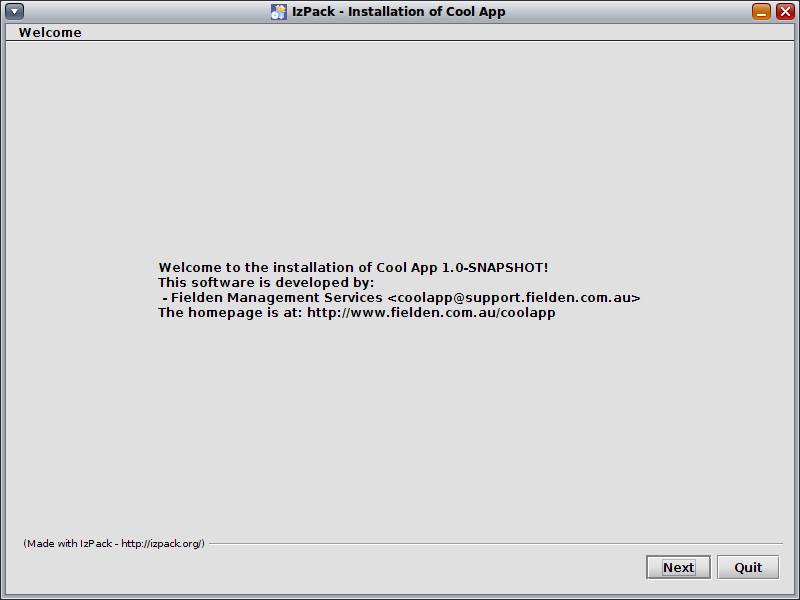
\includegraphics[width=0.6\textwidth]{parts/00-part/chapters/01-application-modules/images/01-client-installation.png}
  \end{image}

  \begin{image}{Client documentation provided as part of the installation}{\label{img:ch00:02:client_installation_doc}}    
    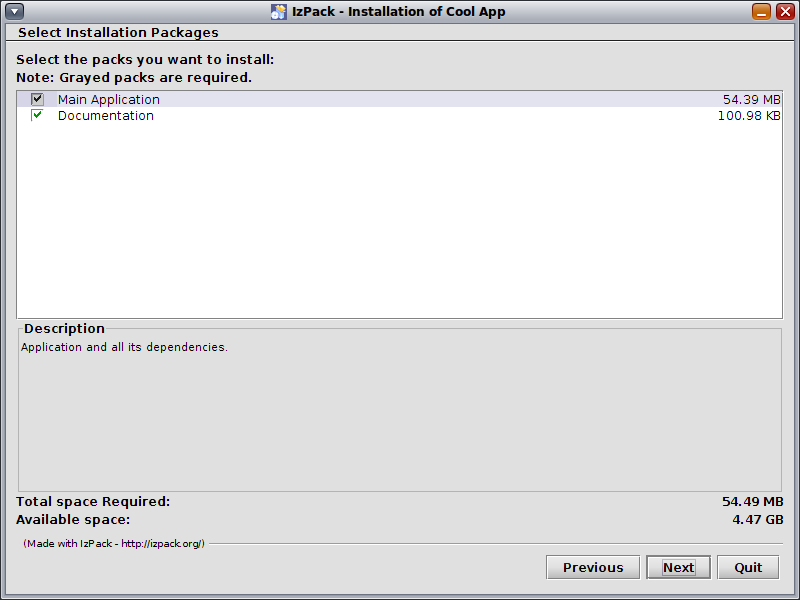
\includegraphics[width=0.6\textwidth]{parts/00-part/chapters/01-application-modules/images/02-client-installation-doc.png}
  \end{image}

  Another important screen is where user needs to specify an application server URI and port.
  The default value is \url{www.fielden.com.au}, but for our purpose due to locally deployed application server, it should be changed to \texttt{localhost} as depicted in Fig.~\ref{img:ch00:02:client_installation_uri}.

  \begin{image}{Application server URI}{\label{img:ch00:02:client_installation_uri}}    
    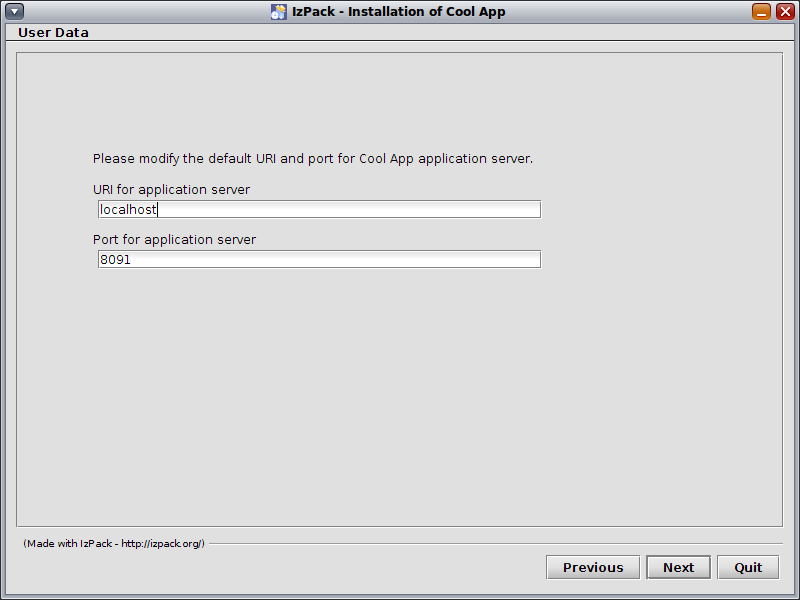
\includegraphics[width=0.6\textwidth]{parts/00-part/chapters/01-application-modules/images/03-client-installation-uri.png}
  \end{image}
  
  Once installation is completed, run the client application by either navigating to the specified installation directory and running \texttt{run.bat} (\texttt{run.sh} for Linux) or by choosing an appropriate program from the \emph{Start} menu under Windows.
  The login screen of the generated application is depicted in Fig.~\ref{img:ch00:02:client_login}.
  The default user name and password is \emph{SU} (both capital).

  \begin{image}{Application login}{\label{img:ch00:02:client_login}}    
    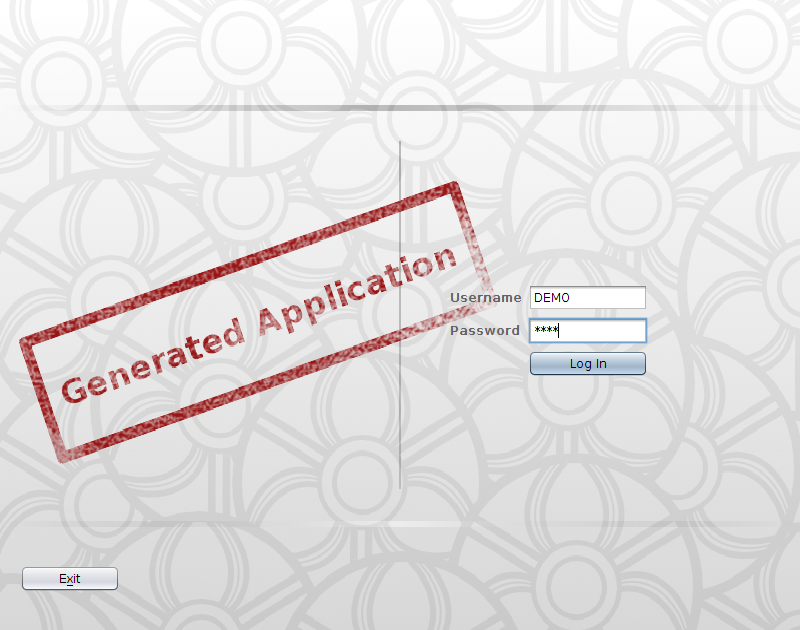
\includegraphics[width=0.6\textwidth]{parts/00-part/chapters/01-application-modules/images/04-client-login.png}
  \end{image}

  The main window of the launched client application is depicted in Fig.~\ref{img:ch00:02:client_main_window}.
  As can be observed, the generated application provides all the necessary functionality for managing users, roles, security tokens as well as the default implementation for \emph{Personnel} and \emph{Attachments}.

  \begin{image}{Application main window}{\label{img:ch00:02:client_main_window}}    
    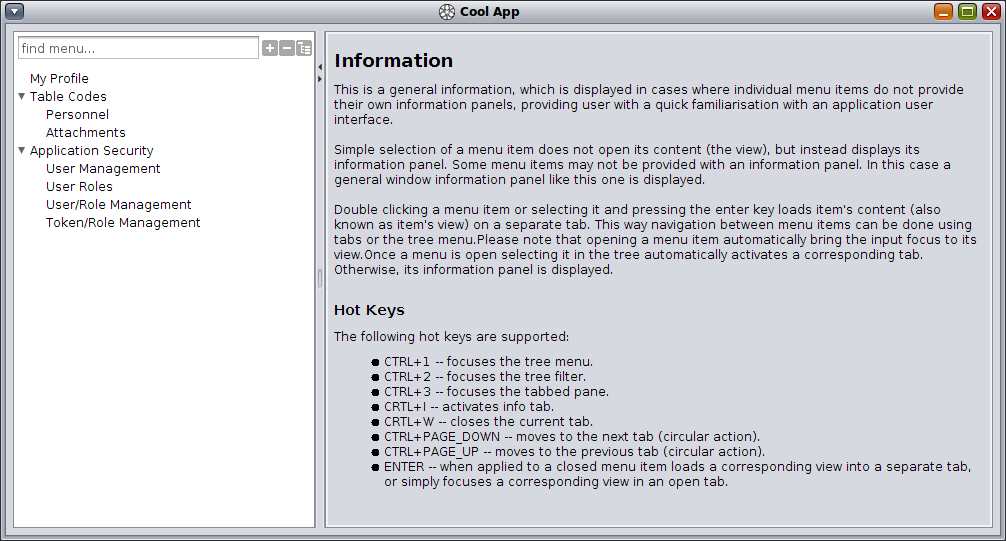
\includegraphics[width=0.7\textwidth]{parts/00-part/chapters/01-application-modules/images/05-client-main-window.png}
  \end{image}

  The above demonstrates how easy it is to start building a TG-based application.
  The provided Trident Genesis Archetype generates a fully operational software with ready to be distributed application server deployment files and a client installation package.
  The use of command line tools for building the project is important as it can be used on headless build servers, which is a common practice in the software industry.

  It is important to note that Trident Genesis Platform offers a complete development methodology, which includes the unified programming model, software distribution model and application documentation creation.
  
  The following sections provide more detailed explanation about the generated application modules, how to set up a development environment and make simple project changes.

\section{Moving to Eclipse}
  It is assumed that the reader is well familiar with Eclipse IDE.
  For developing applications with Trident Genesis we recommend using \href{http://www.eclipse.org/downloads}{Eclipse IDE for Java Developers} as it provides just the right combination of features without introducing unnecessary dependencies.
  The following Plugins are recommended, but not critical, to be installed before starting TG-based application development with Eclipse.

  \begin{description}
    \item[\href{http://www.eclipse.org/m2e/}{M2E}] \hfill \\
	Provides Maven integration with Eclipse. 
	Very useful for analysis and editing of Project Object Model files.
	Sets the \texttt{M2\_REPO} classpath variable pointing to a local Maven repository, which otherwise needs to be created manually.
    \item[\href{http://www.eclipse.org/egit/}{EGit}] \hfill \\
	Provides Git SCM integration with Eclipse. 
	Git is recommended as the preferred source control management system. 
	This plugin ensures correct recognition of various refactorings (e.g. class name refactoring) by Git.
  \end{description}

  In case where for some reason it was decided not to install the M2E plugin, please ensure that the \texttt{M2\_REPO} classpath variable needs to be created in order to properly resolve locations of project dependencies. 
  Figure~\ref{img:ch00:02:m2_repo} depicts such configuration.

  \begin{image}{Setting Eclipse \texttt{M2\_REPO} classpath variable}{\label{img:ch00:02:m2_repo}}    
    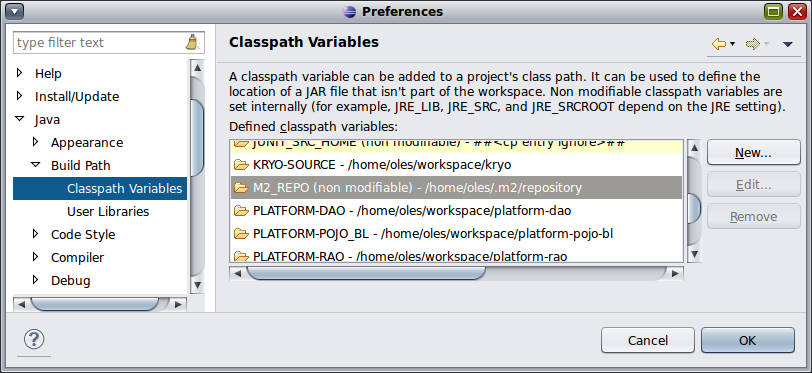
\includegraphics[width=0.9\textwidth]{parts/00-part/chapters/01-application-modules/images/06-eclipse-m2-variable.png}
  \end{image}

\subsection{Generating Eclipse Project}

  In order to make the generated \emph{Cool App} project recognisable by Eclipse IDE, it is necessary to created Eclipse specific project files.
  Conveniently Maven also automates this process.
  Navigate to the project directory \emph{coolapp}, and run the command in listing~\ref{lst:gen_eclipse} to produce all necessary Eclipse files.
  
  \begin{code}{Maven command to generate Eclipse project}{\label{lst:gen_eclipse}}{terminalbgcolor}
     \begin{lstlisting}
user@workstation:~/workspace-tg-apps/coolapp$ mvn -DdownloadSources="true" \
> -DdownloadJavadocs="true" eclipse:eclipse
     \end{lstlisting}
  \end{code}
    
  Options \texttt{downloadSources} and \texttt{downloadJavadocs} ensure that all project dependencies are downloaded with their source and documentation if available.
  This provides developers with capability to read API documentation and even review some of the implementation details from within Eclipse IDE.
  Also, having the source code of project dependencies is crucial in some cases for debugging purposes.

  If the command executed successfully then it should end with the result depicted in listing~\ref{lst:mvn_eclipse_eclipse_completed}. 
  The generated Eclipse project files contain references to all declared in POM dependencies, which use the \texttt{M2\_REPO} classpath variable value to ensure relative paths.

  \begin{notebox}{Project Object Model is primary.}{\label{mb:maven_primary}}
    Remember that POM is the primary source of information for governing the project.
    Therefore, any changes to project dependencies must be done by manipulating project POM files, which may require regeneration of the Eclipse specific files by running the same single command.
  \end{notebox}
  
  \begin{code}{Successful Eclipse project generation}{\label{lst:mvn_eclipse_eclipse_completed}}{terminalbgcolor}
      \begin{lstlisting}
[INFO] ------------------------------------------------------------------------
[INFO] Reactor Summary:
[INFO] ------------------------------------------------------------------------
[INFO] Cool App Parent Project ............................... SUCCESS [3.206s]
[INFO] Cool App POJOs and Business Logic Module .............. SUCCESS [0.538s]
[INFO] Cool App DAO Module ................................... SUCCESS [0.430s]
[INFO] Cool App UI Module .................................... SUCCESS [0.656s]
[INFO] Cool App RAO Module ................................... SUCCESS [0.353s]
[INFO] Cool App Web Client Module ............................ SUCCESS [0.810s]
[INFO] Cool App Web Server Module ............................ SUCCESS [0.390s]
[INFO] ------------------------------------------------------------------------
[INFO] ------------------------------------------------------------------------
[INFO] BUILD SUCCESSFUL
[INFO] ------------------------------------------------------------------------
[INFO] Total time: 7 seconds
[INFO] Finished at: Thu Mar 15 12:13:18 EET 2012
[INFO] Final Memory: 28M/175M
[INFO] ------------------------------------------------------------------------
user@workstation:~/workspace-tg-apps/coolapp$ 
      \end{lstlisting}
  \end{code}

  Now it is time to import the project into Eclipse IDE.

\subsection{Importing Project into Eclipse}

  First what needs to be done is to start Eclipse IDE with workspace directory pointing to \texttt{$\sim$/workspace-tg-apps/} where the generated \texttt{coolapp} project is located.
  Figure~\ref{img:ch00:02:eclipse_workspace} depicts selection of directory \texttt{$\sim$/workspace-tg-apps} as the workspace.  

  \begin{image}{Eclipse Workspace}{\label{img:ch00:02:eclipse_workspace}}    
    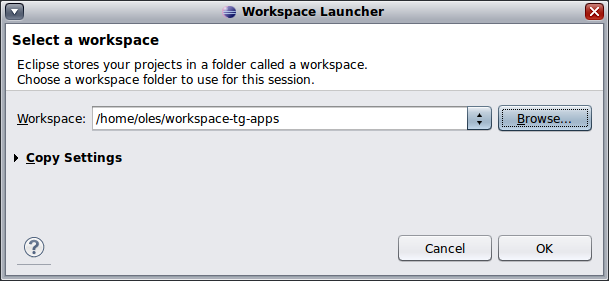
\includegraphics[width=0.9\textwidth]{parts/00-part/chapters/01-application-modules/images/07-eclipse-workspace.png}
  \end{image}

  Once Eclipse has finished loading, choose the \emph{Java Perspective} and use the \emph{Import\ldots} option to initiate the project import as depicted in Fig.~\ref{img:ch00:02:eclipse_importing}.
  
  \begin{image}{Initiating Eclipse Import}{\label{img:ch00:02:eclipse_importing}}    
    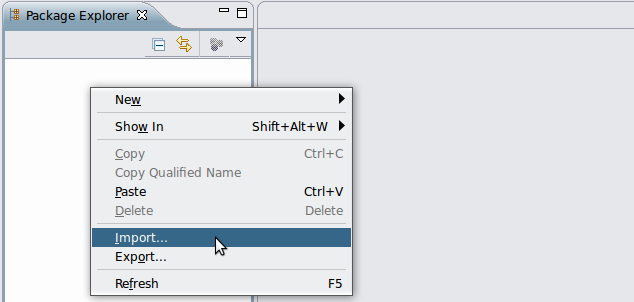
\includegraphics[width=0.95\textwidth]{parts/00-part/chapters/01-application-modules/images/08-eclipse-importing.png}
  \end{image}

  In the \emph{Import} dialog choose \emph{Existing Projects into Workspace} as depicted in Fig.~\ref{img:ch00:02:eclipse_importing_existing}.

  \begin{image}{Import Existing Project into Workspace}{\label{img:ch00:02:eclipse_importing_existing}}        
    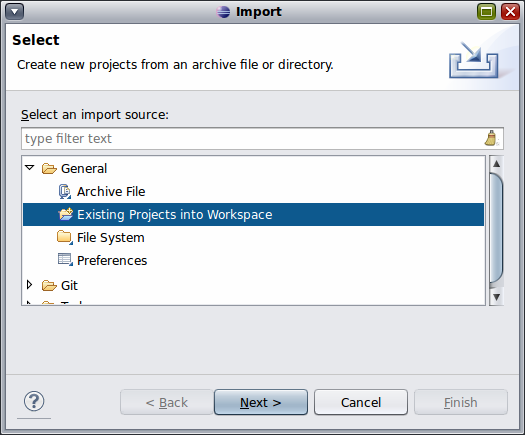
\includegraphics[width=0.6\textwidth]{parts/00-part/chapters/01-application-modules/images/09-eclipse-importing.png}
  \end{image}

  In the next dialog \emph{Brows\ldots} to select \texttt{coolapp} directory as root.
  The result of this action should be the appearance of all project modules in the \emph{Projects} list as depicted in Fig.~\ref{img:ch00:02:eclipse_importing_root}.  
  Therefore, each project module is recognised by Eclipse IDE as a separate project.
  
  Eclipse supports the notion of project dependencies where different projects may have other projects in their class path.
  This is the mechanism by which Maven resolves the dependencies between project modules at the source code level.
  So any design time changes in any module are immediately visible to any other project module that depends on the changed one.

  Click the \emph{Finish} button to complete the import process.
  As the result there should be six separate Eclipse projects representing the project modules visible in \emph{Package Explorer} as depicted in Fig.~\ref{img:ch00:02:eclipse_imported_modules}.
  The imported modules are automatically compiled and if all dependencies are resolved correctly there should be no compilation errors.

  \begin{image}{Select \texttt{coolapp} Directory as Root}{\label{img:ch00:02:eclipse_importing_root}}    
    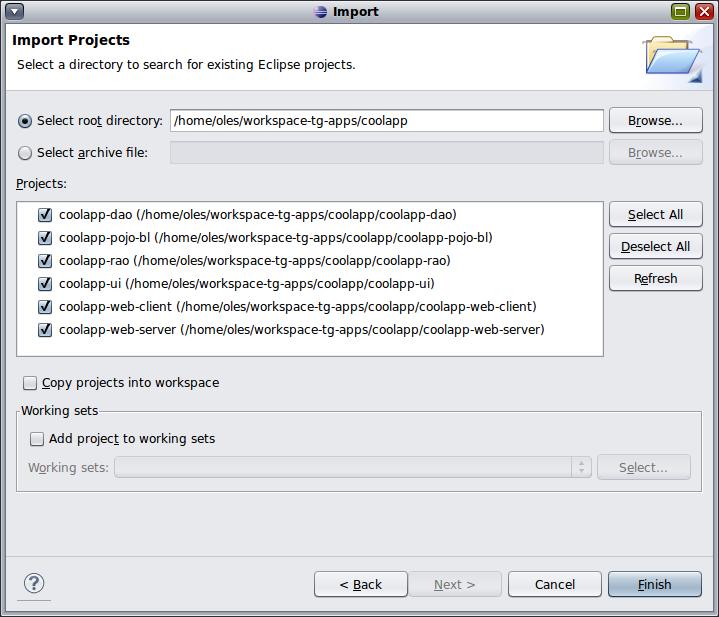
\includegraphics[width=0.7\textwidth]{parts/00-part/chapters/01-application-modules/images/10-eclipse-importing.png}
  \end{image}
 
  \begin{image}{Imported Modules}{\label{img:ch00:02:eclipse_imported_modules}}    
    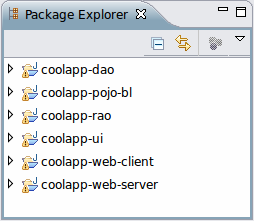
\includegraphics[width=0.4\textwidth]{parts/00-part/chapters/01-application-modules/images/11-eclipse-imported-modules.png}
  \end{image}  
 

  The next step is setup \emph{Run} configurations in order to be able running both application server and client from inside of Eclipse IDE.
  The following section walks through this process.

\subsection{Setting up Run Configurations}

  In order to run application server and client from Eclipse, there is no need to build and package project modules.
  The compilation process is fully incremental in Eclipse, which makes every change to the source code affective almost instantaneously.
  And packaging is not needed as there is no need to deploy anything.

  \subsubsection*{Server}
  The application server is represented by project \texttt{coolapp-web-server}.
  In order to start the server a \emph{Run} configuration needs to be created for this project.
  
  Go to main Eclipse menu \emph{Run} and select \emph{Run Configurations\ldots} to start the configuration dialog.
  Select item \emph{Java Application} in the tree on the left-hand side of the dialog and click the \emph{New launch configuration} (\tikz[baseline=-5pt]\node (V) {
\includegraphics{parts/00-part/chapters/01-application-modules/images/12-server-module-run-config-new-button.png}};) button located on the left side of the toolbox above the tree.
  Provide the configuration with sensible name such as \emph{Cool App Server}, which can be done in the panel on the right-hand side of the dialog.
  Specify value \emph{coolapp-web-server} for the \emph{Project} field (or select is from the list provided once the \emph{Browse\ldots} button is clicked).
  The \emph{Main class} value should be set to \emph{fielden.webapp.StartAsWebinf}.
  Figure~\ref{img:ch00:02:server-module-run-config-main-tab} depicts such configuration.  

  \begin{image}{Cool App Server Run Configuration (Main)}{\label{img:ch00:02:server-module-run-config-main-tab}}    
    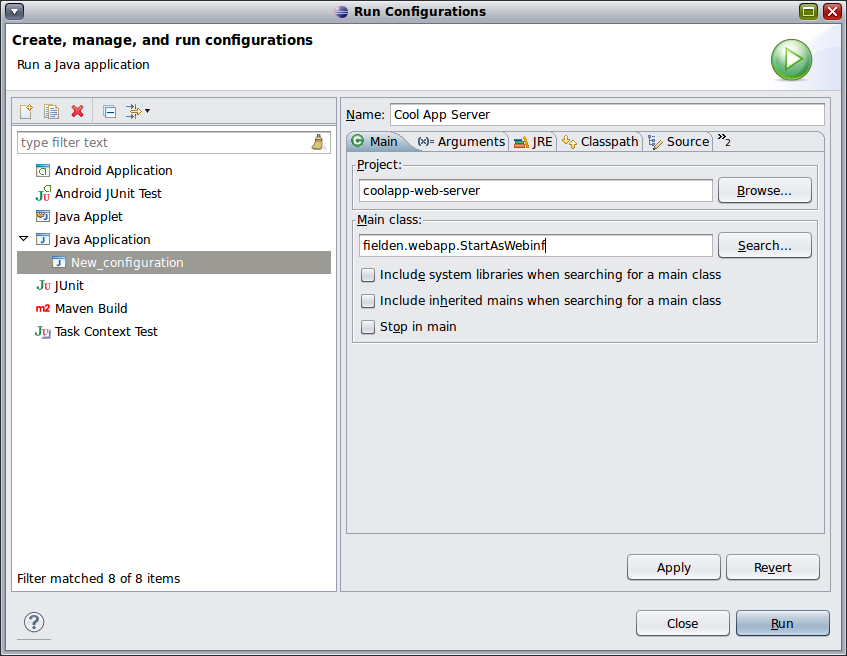
\includegraphics[width=0.75\textwidth]{parts/00-part/chapters/01-application-modules/images/13-server-module-run-config-main-tab.png}
  \end{image}

  The application server needs requires a number of settings such as what database should be used, on port to listen and more.
  The generated project contains all of these settings as part of file \emph{application.properties} located at the root of the module.
  In order to specify this file select tabsheet \emph{Arguments} and set the value of \emph{Program arguments} to \emph{application.properties} as depicted in Fig.~\ref{img:ch00:02:server-module-run-config-args-tab}.
  Once that is done press the \emph{Run} button in the bottom right corner of the dialog to start the server.
  As the result, the \emph{Console} tabsheet of the Java perspective in Eclipse IDE should contain an output, which indicates a successful server launch.
  
  The next step is to run the client application.

  \begin{image}{Cool App Server Run Configuration (Arguments)}{\label{img:ch00:02:server-module-run-config-args-tab}}    
    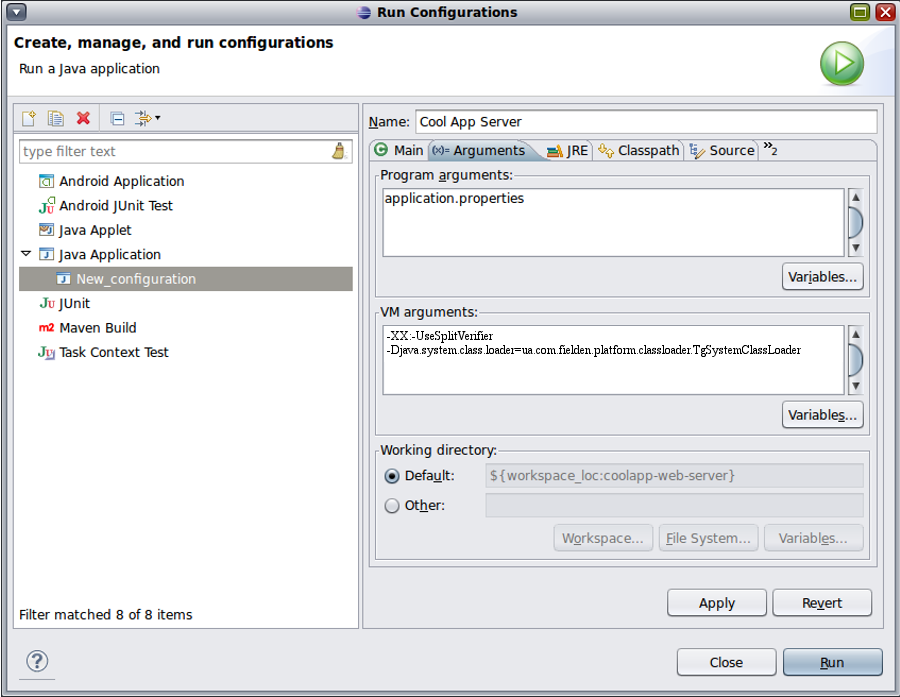
\includegraphics[width=0.75\textwidth]{parts/00-part/chapters/01-application-modules/images/14-server-module-run-config-arguments-tab.png}
  \end{image}
  

  \subsubsection*{Client}
  
  The client application is represented by project \texttt{coolapp-web-client}.
  Setting up a \emph{Run} configuration for it is very similar to the above.
  Navigate to the main menu item \emph{Run} and select \emph{Run Configurations\ldots} to start the configuration dialog.
  Select item \emph{Java Application} in the tree on the left-hand side of the dialog and click the \emph{New launch configuration} (\tikz[baseline=-5pt]\node (V) {
\includegraphics{parts/00-part/chapters/01-application-modules/images/12-server-module-run-config-new-button.png}};) button located as before.
  Provide the configuration with sensible name such as \emph{Cool App Client}.
  Specify value \emph{coolapp-web-client} for the \emph{Project} field (or select is from the list provided once the \emph{Browse\ldots} button is clicked).
  The \emph{Main class} value should be set to \emph{fielden.client.web.ApplicationWebClient}.
  Figure~\ref{img:ch00:02:client-module-run-config-main-tab} depicts such configuration.  

  \begin{image}{Cool App Client Run Configuration (Main)}{\label{img:ch00:02:client-module-run-config-main-tab}}    
    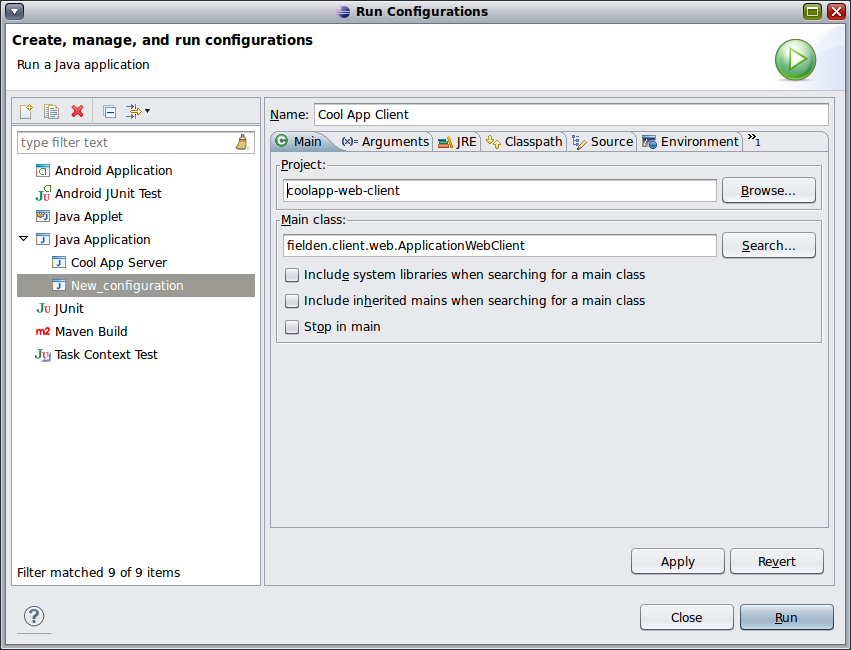
\includegraphics[width=0.75\textwidth]{parts/00-part/chapters/01-application-modules/images/15-client-module-run-config-main-tab.png}
  \end{image}

  The client application also requires a number of settings such as application server URI, a directory for persisting client specific data and more.
  The generated project contains all of these settings as part of file \emph{application.properties} located at the root of the client application module.
  Please note that this is a different file to the one used for an application server albeit its identical name.
  As before select tabsheet \emph{Arguments} and set the value of \emph{Program arguments} to \emph{application.properties} as depicted in Fig.~\ref{img:ch00:02:client-module-run-config-arguments-tab}.
  Additionally, the client module is provided with branding support, which includes a splash screen.
  The splash screen should be specified as value \emph{-splash:src/main/resources/images/splash.jpg} for \emph{VM Arguments} on the same \emph{Arguments} tabsheet.
  Once all these settings are provided, press the \emph{Run} button in the bottom right corner of the dialog to start the client.
  If everything was configured correctly and the application server is running, then first a splash screen should appear on the screen followed by the login prompt.
  The client application itself is identical to the one observed in section~\ref{ch00:02:client}.

  \begin{image}{Cool App Client Run Configuration (Arguments)}{\label{img:ch00:02:client-module-run-config-arguments-tab}}    
    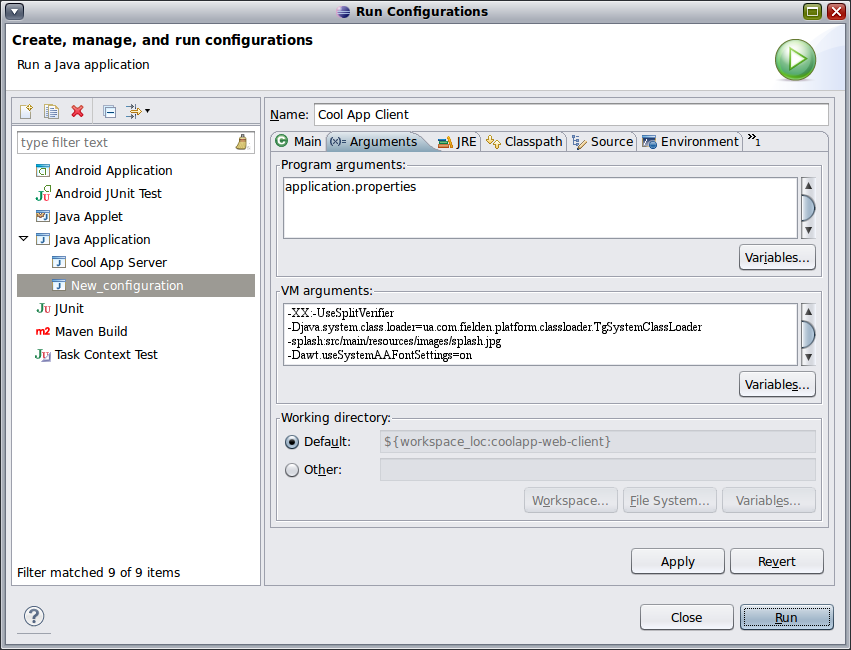
\includegraphics[width=0.75\textwidth]{parts/00-part/chapters/01-application-modules/images/16-client-module-run-config-arguments-tab.png}
  \end{image}

  Hopefully by now the reader could see how quickly it was to start a TG-based project with a complete automation of the processes to build and deploy the application as well as to configure the development environment.
  
  It's about time to make some project changes and see easy it is.
  These discussed changes are trivial for the purpose of keep the quick start\ldots well\ldots quick, and a more elaborate discussion of various platform approaches to domain modelling, UI construction and more will be presented in later chapters of the book.